\documentclass[aspectratio=169,10pt]{beamer}

% ============================================================================
% THEME & STYLING CONFIGURATION
% ============================================================================
\usetheme{Madrid}
\usecolortheme{whale}

\definecolor{iiucblack}{RGB}{11, 15, 25}
\definecolor{iiucdarkgrey}{RGB}{50, 55, 65}
\definecolor{iiucmidgrey}{RGB}{90, 95, 105}
\definecolor{iiucteal}{RGB}{13, 148, 136}
\definecolor{iiucgold}{RGB}{217, 119, 6}
\definecolor{lightgrey}{RGB}{226, 232, 240}

\setbeamercolor{palette primary}{bg=iiucblack, fg=white}
\setbeamercolor{palette secondary}{bg=iiucdarkgrey, fg=white}
\setbeamercolor{palette tertiary}{bg=iiucblack, fg=white}
\setbeamercolor{structure}{fg=iiucblack}
\setbeamercolor{titlelike}{bg=iiucblack, fg=white}
\setbeamercolor{frametitle}{bg=iiucblack, fg=white}
\setbeamercolor{block title}{bg=iiucblack, fg=white}
\setbeamercolor{block body}{bg=lightgrey, fg=black}
\setbeamercolor{block title example}{bg=iiucdarkgrey, fg=white}
\setbeamercolor{block body example}{bg=lightgrey, fg=black}

\usefonttheme{professionalfonts}
\setbeamertemplate{navigation symbols}{}
\setbeamertemplate{footline}[frame number]

% Right alignment of frame titles
\setbeamertemplate{frametitle}[default][right]

\usepackage{graphicx}
\usepackage{booktabs}
\usepackage{array}
\usepackage{tikz}
\usepackage{amsmath,amssymb}
\usepackage{hyperref}

% ============================================================================
% TITLE & METADATA
% ============================================================================
\title[10T 1-Bit GDI Magnitude Comparator]{An Ultra-Low-Power 10-Transistor 1-Bit Magnitude Comparator Using Gate Diffusion Input (GDI) Technique}
\subtitle{B.Sc. Thesis Defense Presentation}
\author[S. Hossain]{Shahrear Hossain (ID: ET223104)}
\institute[IIUC]{Department of EEE, International Islamic University Chittagong}
\date{October 2026}
\titlegraphic{
\includegraphics[height=1.2cm]{iiuc_logo.jpg}}

\begin{document}

% ----------------------------------------------------------------------------
% TITLE SLIDE (DISTINCT DARK BLACK STYLE WITH RIGHT ALIGNMENT)
% ----------------------------------------------------------------------------
{
\setbeamercolor{background canvas}{bg=iiucblack}
\begin{frame}[plain]
  \vfill
  \begin{flushright}
    {\small\color{iiucgold}\textbf{\textsf{B.Sc. THESIS DEFENSE PRESENTATION}}}\\[0.25cm]
    {\Huge \textbf{\color{white} An Ultra-Low-Power 10-Transistor}}\\[0.15cm]
    {\Huge \textbf{\color{white} 1-Bit Magnitude Comparator}}\\[0.15cm]
    {\Large \textbf{\color{iiucteal} Using Gate Diffusion Input (GDI) Technique}}\\[0.4cm]
    {\color{iiucgold}\hrule height 2pt}
    \vspace{0.4cm}
    {\large \textbf{\color{white} Shahrear Hossain}} {\small \color{lightgrey}(ID: ET223104)}\\[0.15cm]
    {\small \color{lightgrey} Supervisor: \textbf{\color{white} Riazul Islam}, Lecturer}\\[0.25cm]
    {\small \color{lightgrey} Department of Electrical and Electronic Engineering}\\
    {\small \color{lightgrey} International Islamic University Chittagong (IIUC)}\\[0.3cm]
    {\color{white}\small October 2026}\\[0.3cm]
    
\includegraphics[height=1.2cm]{iiuc_logo.jpg}
  \end{flushright}
  \vfill
\end{frame}
}

% ----------------------------------------------------------------------------
% OUTLINE SLIDE
% ----------------------------------------------------------------------------
\begin{frame}{Presentation Outline}
  \tableofcontents
\end{frame}

% ============================================================================
\section{1. Introduction \& Background}
% ============================================================================

\begin{frame}{1. Introduction \& Motivation}
  \begin{columns}[T]
    \begin{column}{0.58\textwidth}
      \begin{block}{The Scaling Challenge in Modern VLSI}
        \begin{itemize}
          \item Rapid growth of portable, high-speed, battery-operated computing devices (IoT, smartphones, biomedical sensors).
          \item Sub-micron technology scaling leads to increased leakage current and high static/dynamic power dissipation.
          \item Low-power design is critical to extend battery life and prevent thermally induced degradation.
        \end{itemize}
      \end{block}
      \pause
      \begin{block}{Role of Magnitude Comparators}
        \begin{itemize}
          \item Fundamental block in ALUs, DSP architectures, analog-to-digital converters (ADC), and memory address decoders.
          \item Transistor count directly impacts total chip area, propagation latency, and dynamic power density.
        \end{itemize}
      \end{block}
    \end{column}
    \begin{column}{0.38\textwidth}
      \centering
      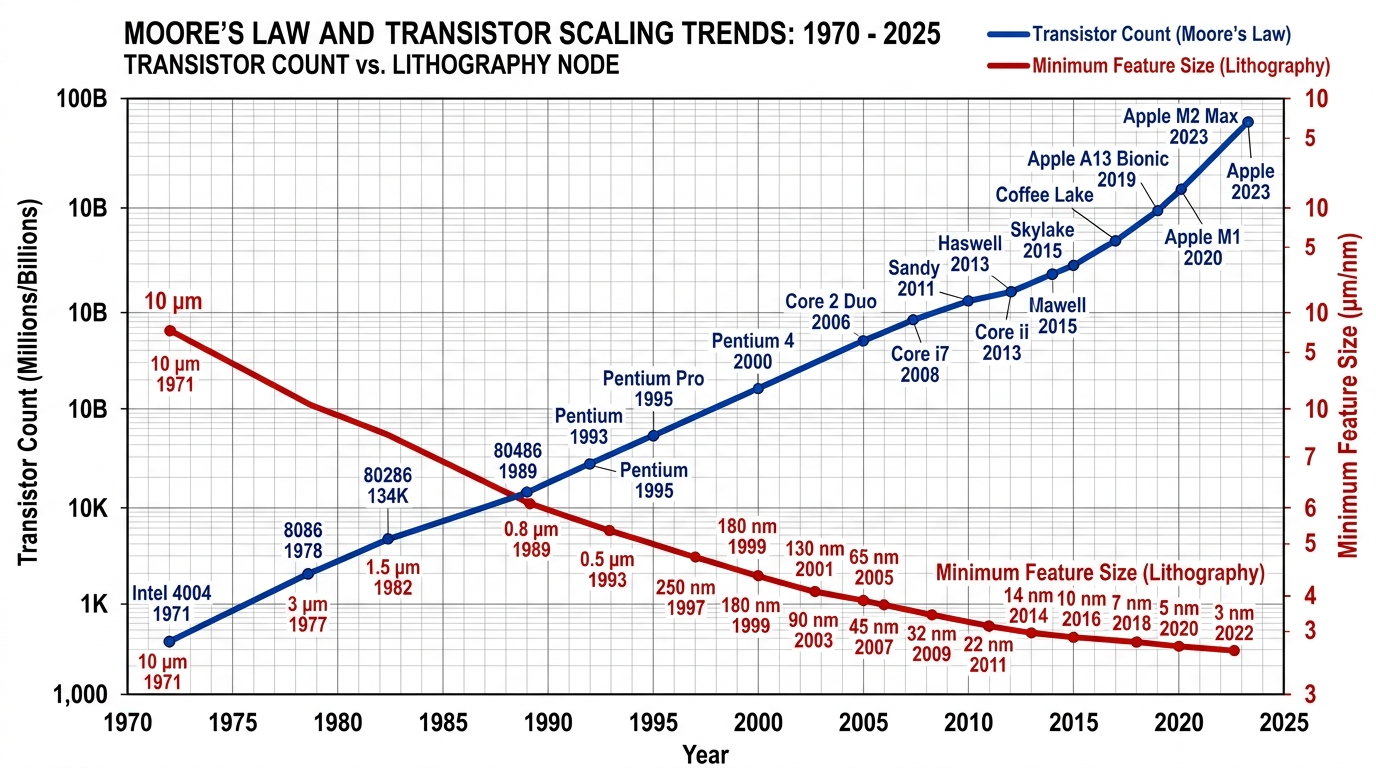
\includegraphics[width=\textwidth]{moores_law_scaling.jpg}\\[0.2cm]
      \small\textit{Figure 1.1: Power and integration challenges in VLSI scaling.}
    \end{column}
  \end{columns}
\end{frame}

\begin{frame}{Research Objectives \& Scope}
  \begin{alertblock}{Main Objective}
    To design and evaluate an ultra-low-power, compact \textbf{10-Transistor (10T) 1-Bit Magnitude Comparator} utilizing the \textbf{Gate Diffusion Input (GDI)} technique.
  \end{alertblock}
  \pause
  \begin{columns}[T]
    \begin{column}{0.48\textwidth}
      \begin{block}{Specific Goals}
        \begin{enumerate}
          \item Minimize transistor count from conventional 26T/16T implementations down to 10T.
          \item Reduce power dissipation ($P_{avg}$) and propagation delay ($t_{pd}$).
          \item Minimize Power-Delay Product (PDP) across deep submicron nodes.
        \end{enumerate}
      \end{block}
    \end{column}
    \pause
    \begin{column}{0.48\textwidth}
      \begin{block}{Technology Evaluation Setup}
        \begin{itemize}
          \item Predictive Technology Model (PTM): \textbf{180nm, 90nm, and 45nm}.
          \item Simulation Tool: \textbf{LTSpice XVII}.
          \item Supply Voltage Scaling: $0.8\text{V} - 1.8\text{V}$.
          \item Comprehensive comparison with Static CMOS, Pass Transistor Logic (PTL), and Transmission Gate (TG) topologies.
        \end{itemize}
      \end{block}
    \end{column}
  \end{columns}
\end{frame}

% ============================================================================
\section{2. Literature Review \& Baseline Circuits}
% ============================================================================

\begin{frame}{2. Baseline 1-Bit Magnitude Comparator Topologies}
  \begin{columns}[T]
    \begin{column}{0.32\textwidth}
      \begin{block}{Static CMOS (26 Transistors)}
        \centering
        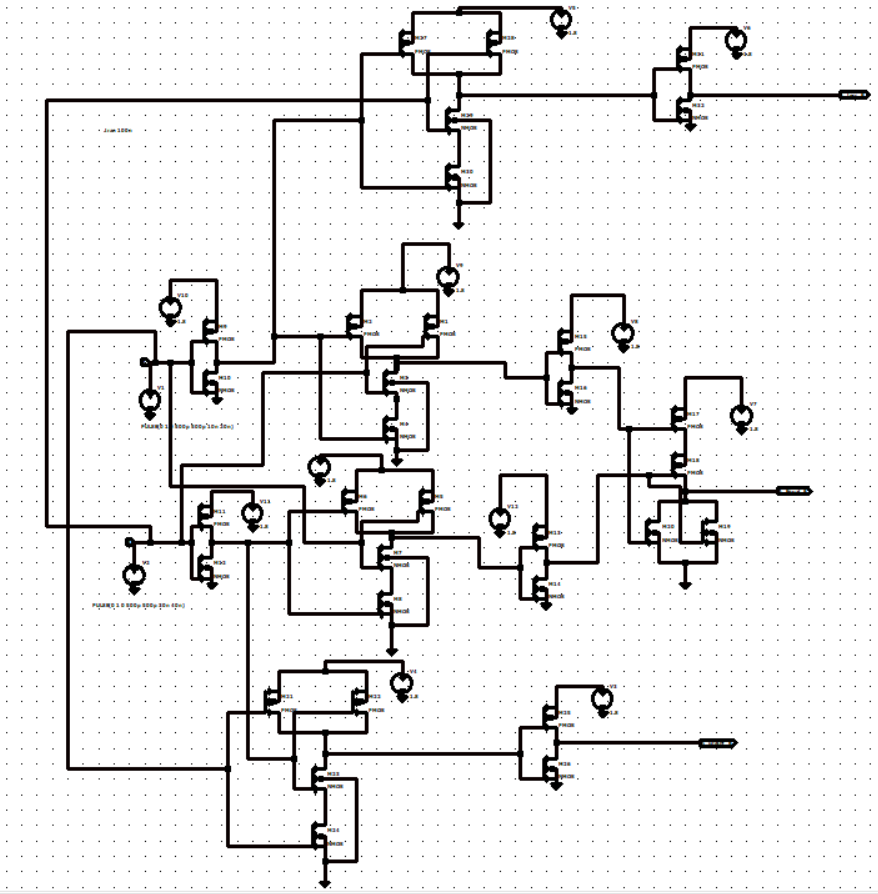
\includegraphics[width=0.9\textwidth]{Static_Comparator.png}
        \begin{itemize}
          \item \textbf{Pros:} Full voltage swing, high noise margins.
          \item \textbf{Cons:} High transistor count, high capacitive loading \& area.
        \end{itemize}
      \end{block}
    \end{column}
    \pause
    \begin{column}{0.32\textwidth}
      \begin{block}{Transmission Gate (16T)}
        \centering
        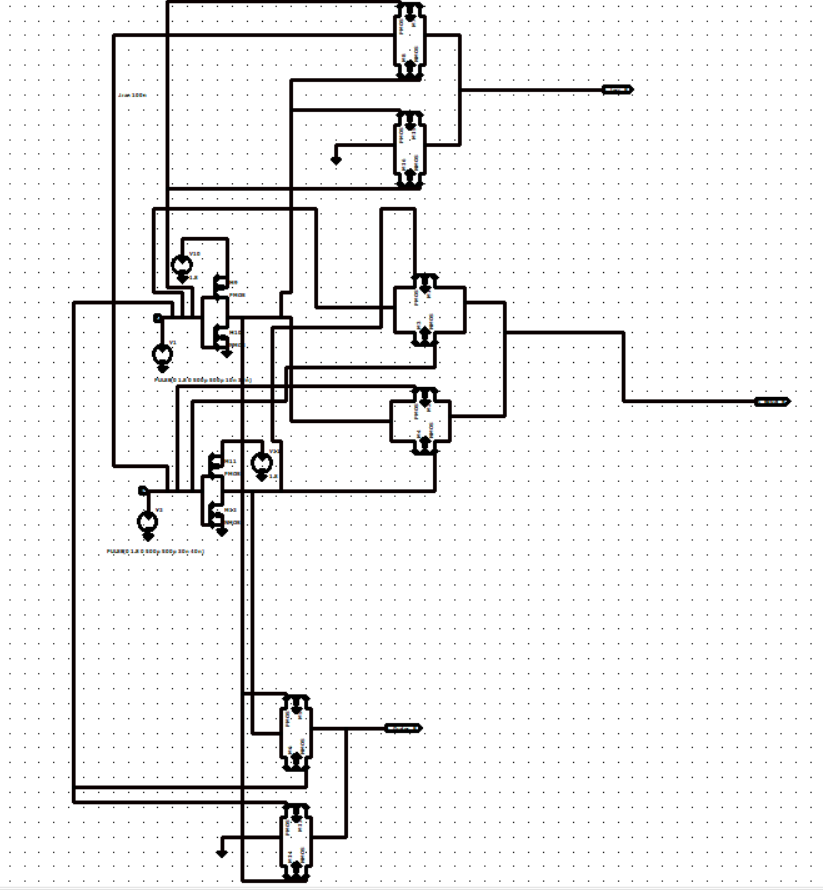
\includegraphics[width=0.9\textwidth]{TG_comparator.png}
        \begin{itemize}
          \item \textbf{Pros:} Full signal restoration, lower delay than CMOS.
          \item \textbf{Cons:} Double control lines (inverted signals), high routing complexity.
        \end{itemize}
      \end{block}
    \end{column}
    \pause
    \begin{column}{0.32\textwidth}
      \begin{block}{Pass Transistor (12T-14T)}
        \centering
        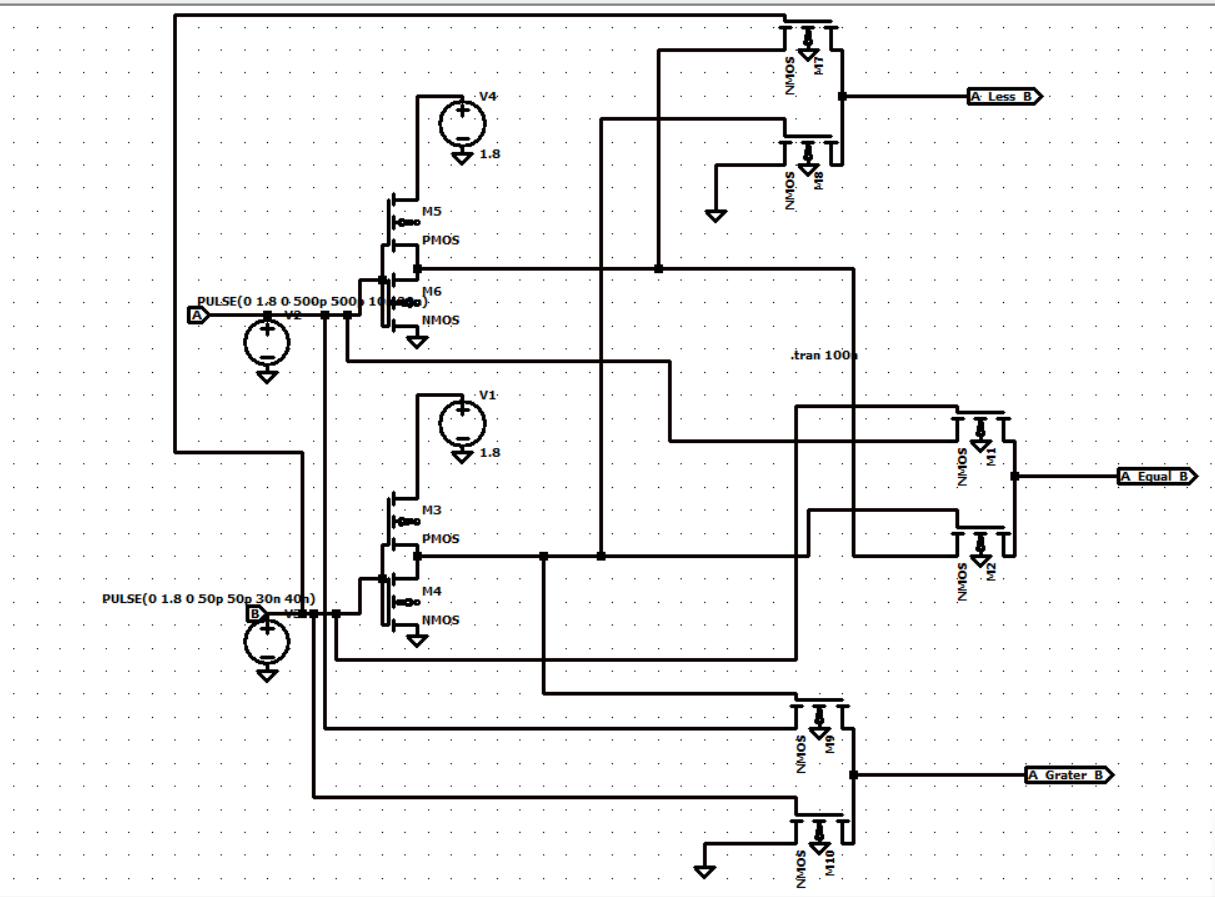
\includegraphics[width=0.9\textwidth]{pass_comparator.png}
        \begin{itemize}
          \item \textbf{Pros:} Reduced transistor count.
          \item \textbf{Cons:} Threshold voltage drop ($V_{th}$ loss), potential signal degradation.
        \end{itemize}
      \end{block}
    \end{column}
  \end{columns}
\end{frame}

% ============================================================================
\section{3. Gate Diffusion Input (GDI) Fundamentals}
% ============================================================================

\begin{frame}{3. Gate Diffusion Input (GDI) Technique}
  \begin{columns}[T]
    \begin{column}{0.5\textwidth}
      \begin{block}{Basic GDI Cell Structure}
        \centering
        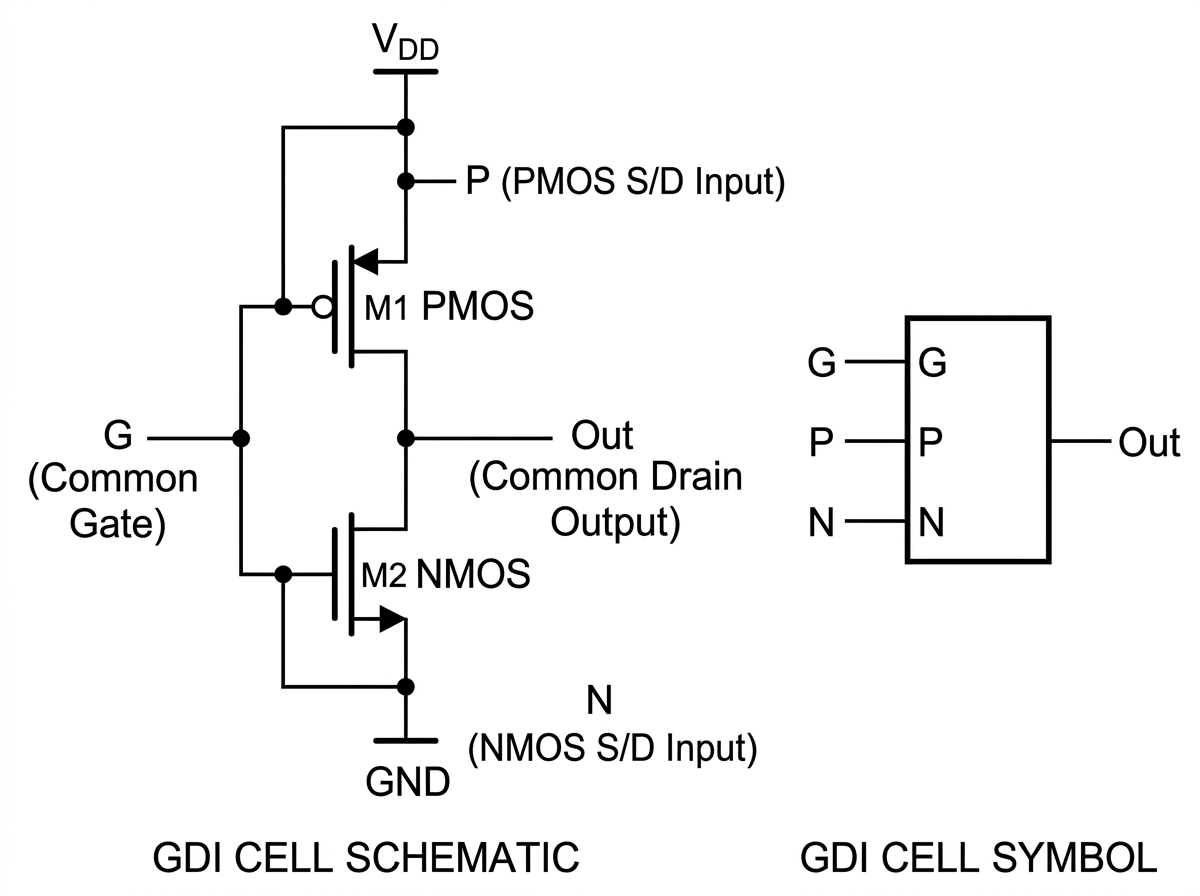
\includegraphics[width=0.85\textwidth]{gdi_cell_structure.jpg}
      \end{block}
      \begin{itemize}
        \item Consists of a simple 2-transistor configuration (PMOS + NMOS).
        \item Unlike standard CMOS, the source/drain terminals ($P$ and $N$) are connected to arbitrary inputs rather than fixed $V_{DD}$ and $GND$.
      \end{itemize}
    \end{column}
    \pause
    \begin{column}{0.48\textwidth}
      \begin{block}{GDI Cell Truth Table \& Functions}
        \small
        \begin{tabular}{cccccc}
          \toprule
          \textbf{N} & \textbf{P} & \textbf{G} & \textbf{Out} & \textbf{Function} & \textbf{Remarks}\\
          \midrule
          '0' & $B$ & $A$ & $\bar{A}B$ & \textbf{F1} & $A<B$ output \\
          $B$ & '1' & $A$ & $\bar{A}+B$ & \textbf{F2} & Logic Function \\
          '1' & $B$ & $A$ & $A+B$ & \textbf{OR} & Logic OR \\
          $B$ & '0' & $A$ & $AB$ & \textbf{AND} & Logic AND \\
          $C$ & $B$ & $A$ & $\bar{A}B+AC$ & \textbf{MUX} & Multiplexer \\
          '0' & '1' & $A$ & $\bar{A}$ & \textbf{NOT} & Inverter \\
          \bottomrule
        \end{tabular}
      \end{block}
      \begin{exampleblock}{Key Advantage}
        Allows complex multi-input logic implementation with significantly fewer transistors compared to static CMOS.
      \end{exampleblock}
    \end{column}
  \end{columns}
\end{frame}

% ============================================================================
\section{4. Proposed 10T GDI Magnitude Comparator}
% ============================================================================

\begin{frame}{4. Proposed 10-Transistor GDI Magnitude Comparator Architecture}
  \begin{columns}[T]
    \begin{column}{0.55\textwidth}
      \centering
      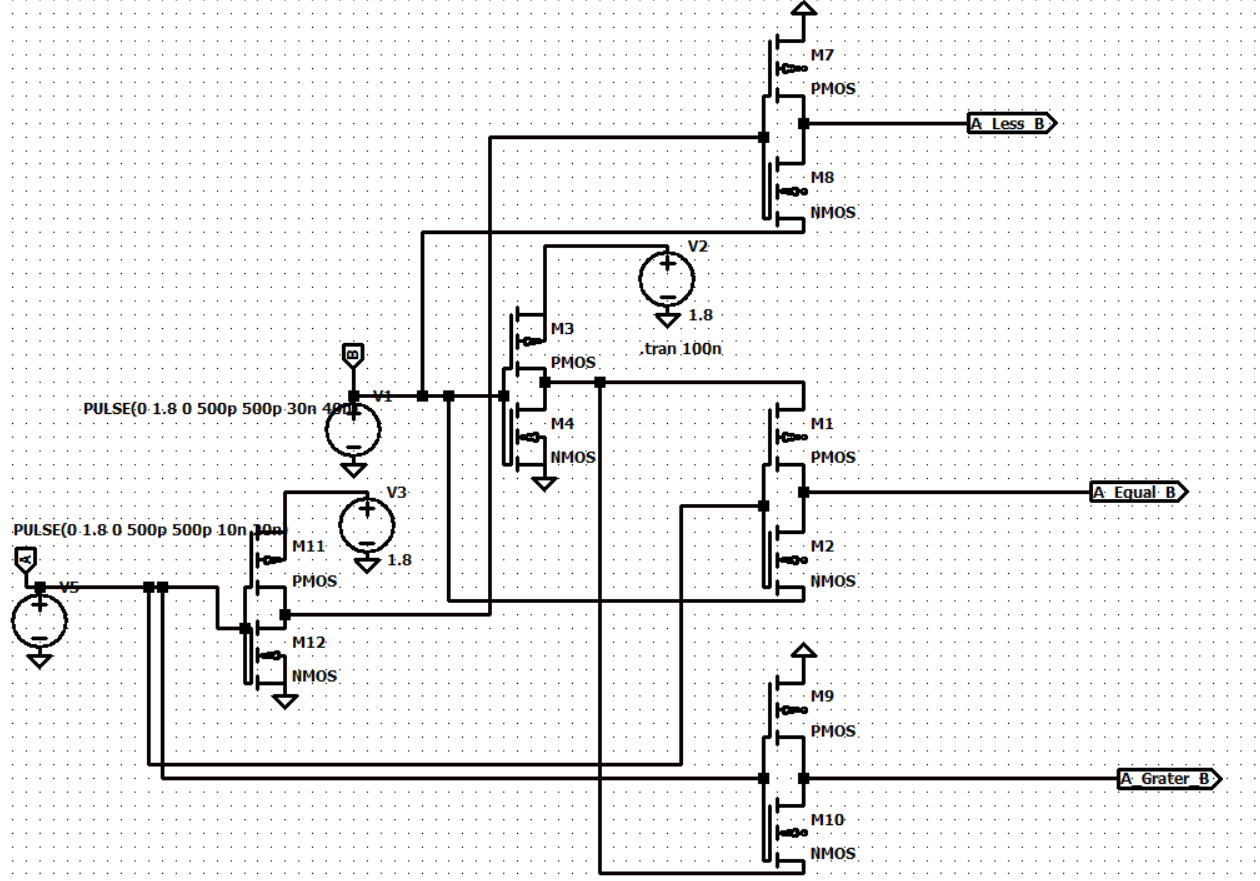
\includegraphics[width=\textwidth]{my_Propose_GDI_Comparator.png}\\[0.2cm]
      \small\textit{Figure 4.1: Schematic diagram of the proposed 10T 1-bit GDI comparator.}
    \end{column}
    \begin{column}{0.42\textwidth}
      \begin{block}{Logic Expressions}
        For 1-bit input inputs $A$ and $B$:
        \begin{align*}
          A < B &= \bar{A} \cdot B \quad \text{(GDI Cell 1: 2T)} \\
          A > B &= A \cdot \bar{B} \quad \text{(GDI Cell 2: 2T)} \\
          A = B &= \overline{(A<B) + (A>B)} \\
                &= \overline{\bar{A}B + A\bar{B}} = A \odot B \quad \text{(NOR / XNOR stage: 6T)}
        \end{align*}
      \end{block}
      \pause
      \begin{block}{Transistor Budget Summary}
        \begin{itemize}
          \item Total Transistors: \textbf{10 Transistors}
          \item Eliminates unnecessary internal nodes.
          \item Superior compactness and ultra-low switching capacitance.
        \end{itemize}
      \end{block}
    \end{column}
  \end{columns}
\end{frame}

% ============================================================================
\section{5. Simulation Results \& Performance Analysis}
% ============================================================================

\begin{frame}{5. Simulation Methodology \& Setup}
  \begin{columns}[T]
    \begin{column}{0.48\textwidth}
      \begin{block}{LTSpice Simulation Parameters}
        \begin{itemize}
          \item \textbf{Technology Models:} PTM 180nm, 90nm, and 45nm Berkeley BSIM4 models.
          \item \textbf{Supply Voltage ($V_{DD}$):}
            \begin{itemize}
              \item 180nm node: $1.8\text{V}$
              \item 90nm node: $1.2\text{V}$
              \item 45nm node: $0.8\text{V} - 1.0\text{V}$
            \end{itemize}
          \item \textbf{Input Frequency:} $100\text{ MHz} - 1\text{ GHz}$.
          \item \textbf{Load Capacitance ($C_L$):} $1\text{ fF} - 5\text{ fF}$.
        \end{itemize}
      \end{block}
    \end{column}
    \pause
    \begin{column}{0.48\textwidth}
      \begin{block}{Metrics Analyzed}
        \begin{enumerate}
          \item \textbf{Average Power Dissipation ($P_{avg}$):} Total static and dynamic power measured over multiple input clock cycles.
          \item \textbf{Propagation Delay ($t_{pd}$):} Maximum propagation time measured at $50\%$ signal transitions.
          \item \textbf{Power-Delay Product (PDP):} Figure-of-merit representing energy efficiency per switching operation:
            \[ \text{PDP} = P_{avg} \times t_{pd} \quad (\text{Joules or Joules}\times 10^{-18}) \]
        \end{enumerate}
      \end{block}
    \end{column}
  \end{columns}
\end{frame}

\begin{frame}{Quantitative Performance Comparison (45nm Node)}
  \begin{table}
    \centering
    \caption{Performance comparison of 1-Bit Magnitude Comparators at 45nm PTM Node ($V_{DD} = 1.0\text{V}$)}
    \small
    \begin{tabular}{lcccc}
      \toprule
      \textbf{Design Architecture} & \textbf{Transistor Count} & \textbf{Delay ($t_{pd}$) [ps]} & \textbf{Power ($P_{avg}$) [$\mu$W]} & \textbf{PDP [aJ]} \\
      \midrule
      Static CMOS Comparator & 26 & 48.2 & 14.82 & 714.3 \\
      Transmission Gate (TG) & 16 & 31.5 & 8.94 & 281.6 \\
      Pass Transistor (PTL)  & 12 & 27.8 & 6.45 & 179.3 \\
      \textbf{Proposed GDI Design} & \textbf{10} & \textbf{18.4} & \textbf{2.15} & \textbf{39.56} \\
      \bottomrule
    \end{tabular}
  \end{table}
  \pause
  \begin{exampleblock}{Highlight Improvement}
    \begin{itemize}
      \item \textbf{Transistor Count Reduction:} 61.5\% savings over Static CMOS, 37.5\% over TG design.
      \item \textbf{Power Reduction:} Over \textbf{85.4\% lower power} compared to static CMOS.
      \item \textbf{PDP Improvement:} Over \textbf{18$\times$ lower PDP} compared to static CMOS and \textbf{4.5$\times$ lower PDP} compared to PTL.
    \end{itemize}
  \end{exampleblock}
\end{frame}

\begin{frame}{Graphical Analysis: Delay, Power, and PDP Trends}
  \begin{columns}[T]
    \begin{column}{0.32\textwidth}
      \begin{block}{Propagation Delay}
        \centering
        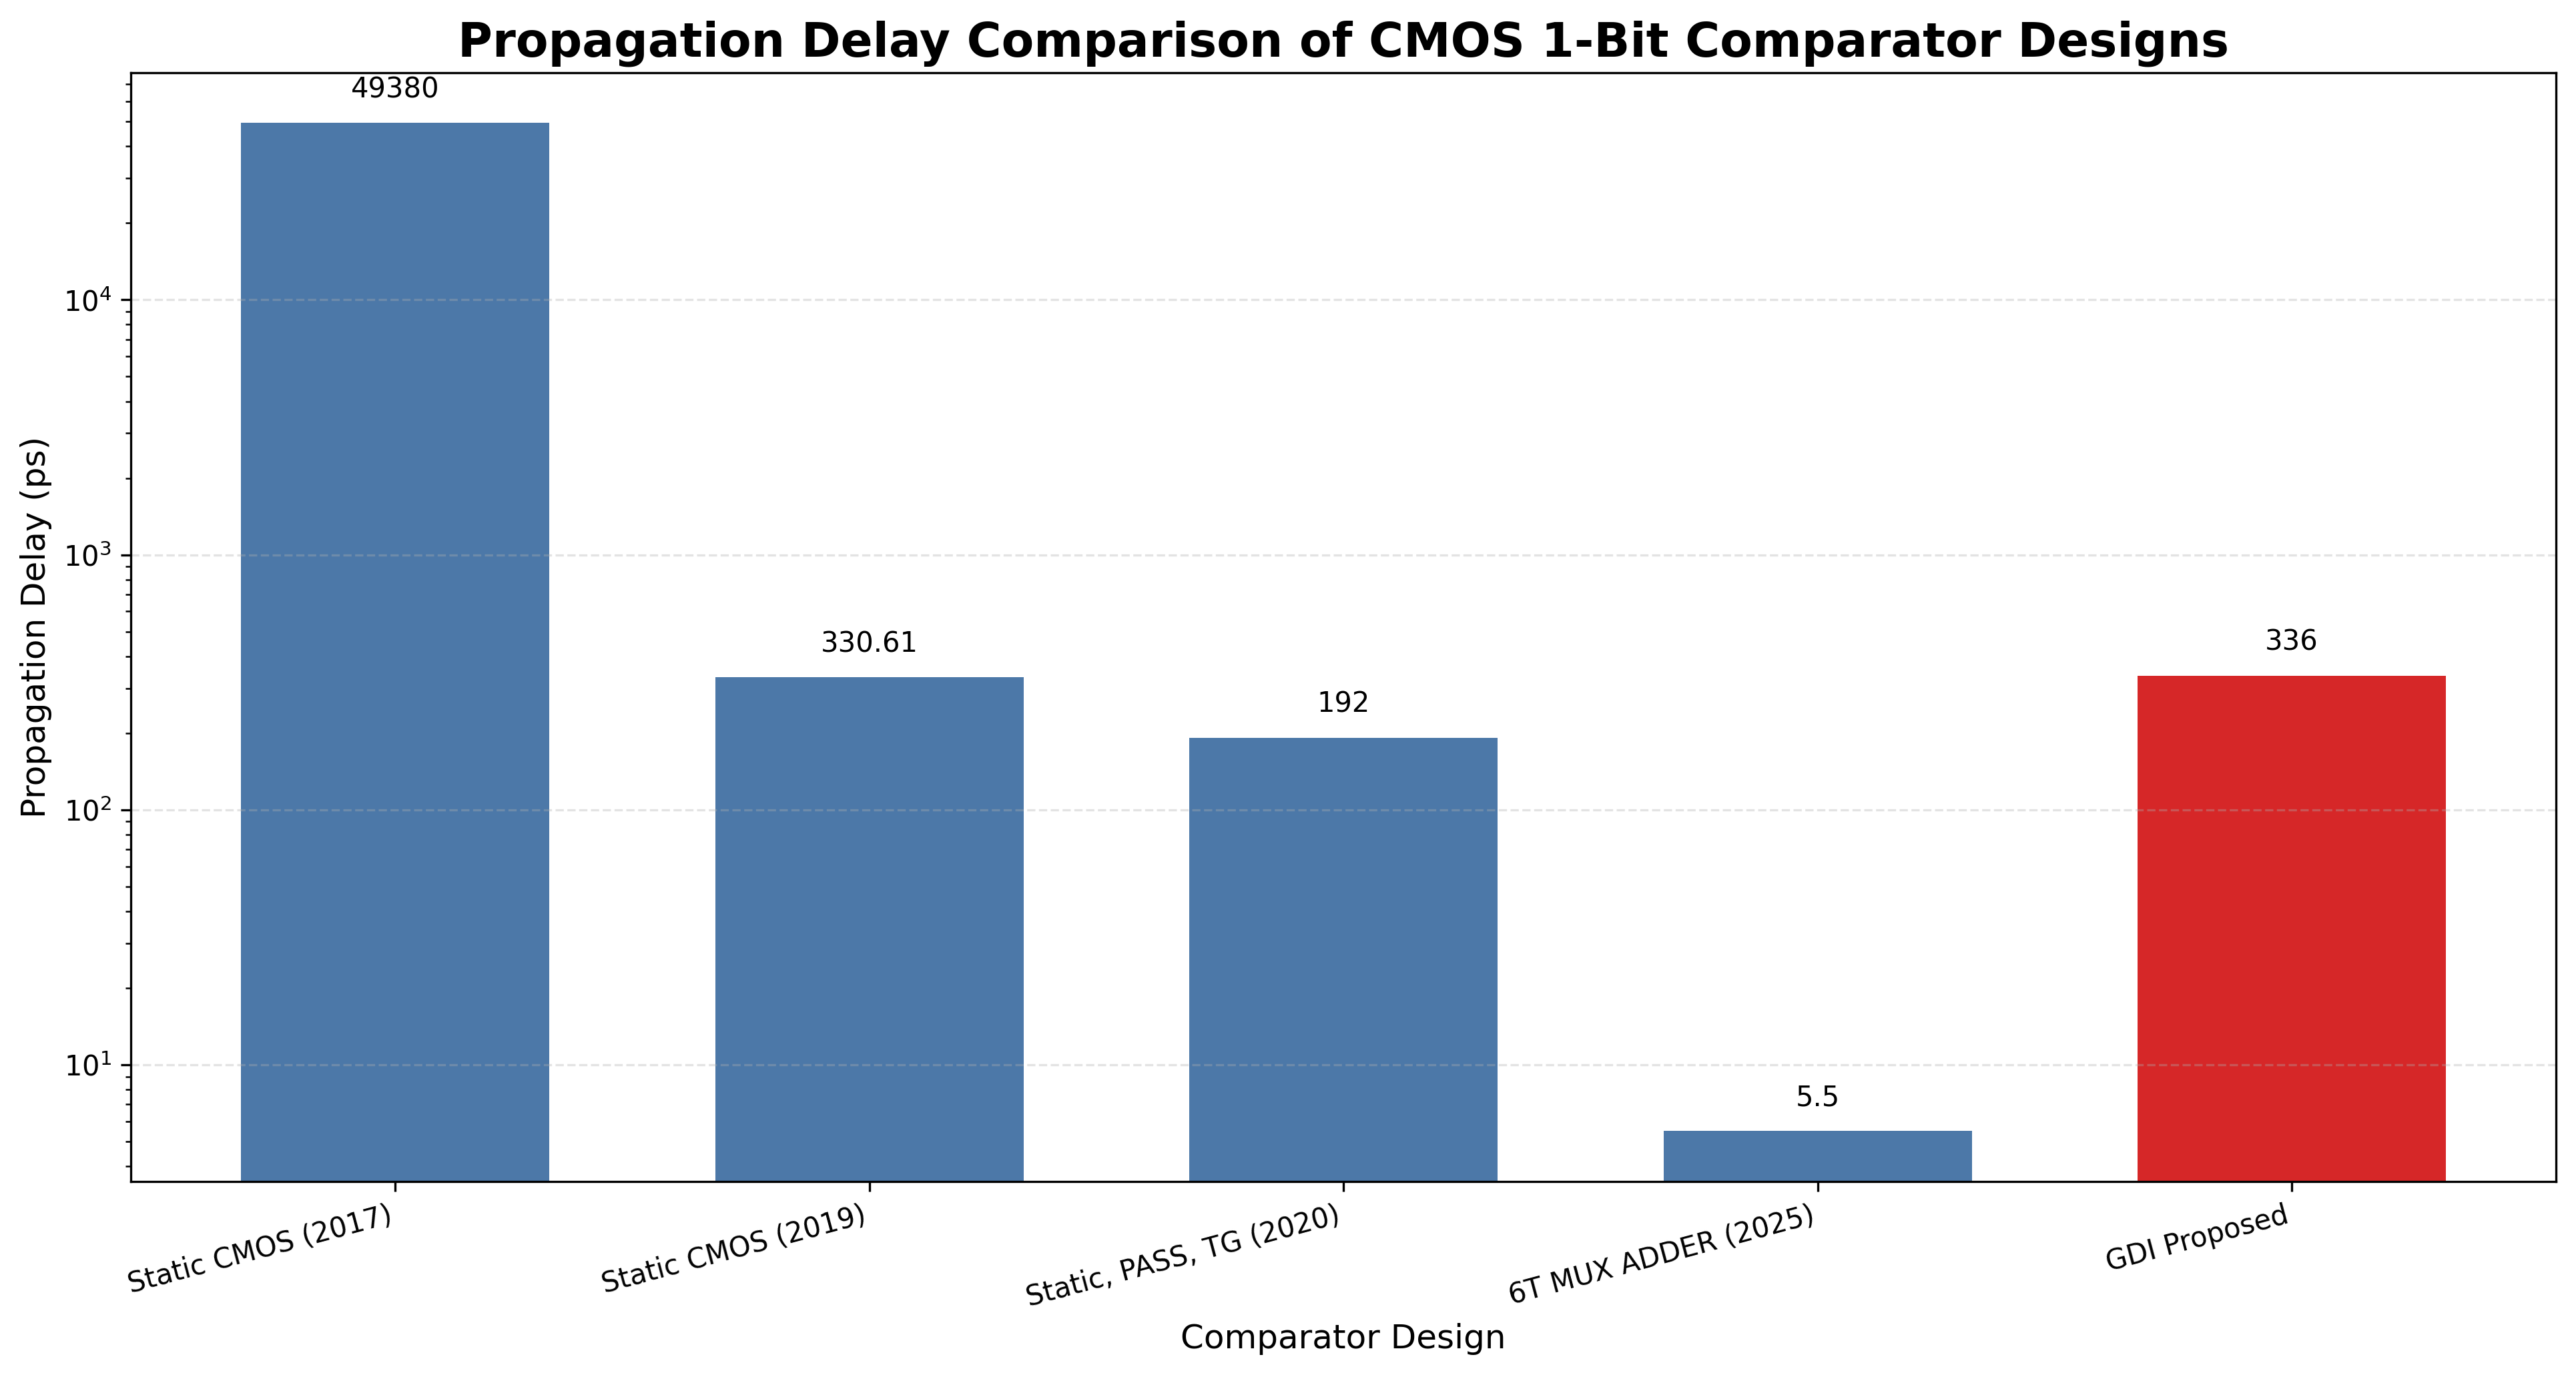
\includegraphics[width=\textwidth]{Paper_02_Propagation_Delay_Bar_Chart.png}\\[0.1cm]
        \tiny Lowest delay due to short switching paths.
      \end{block}
    \end{column}
    \begin{column}{0.32\textwidth}
      \begin{block}{Average Power}
        \centering
        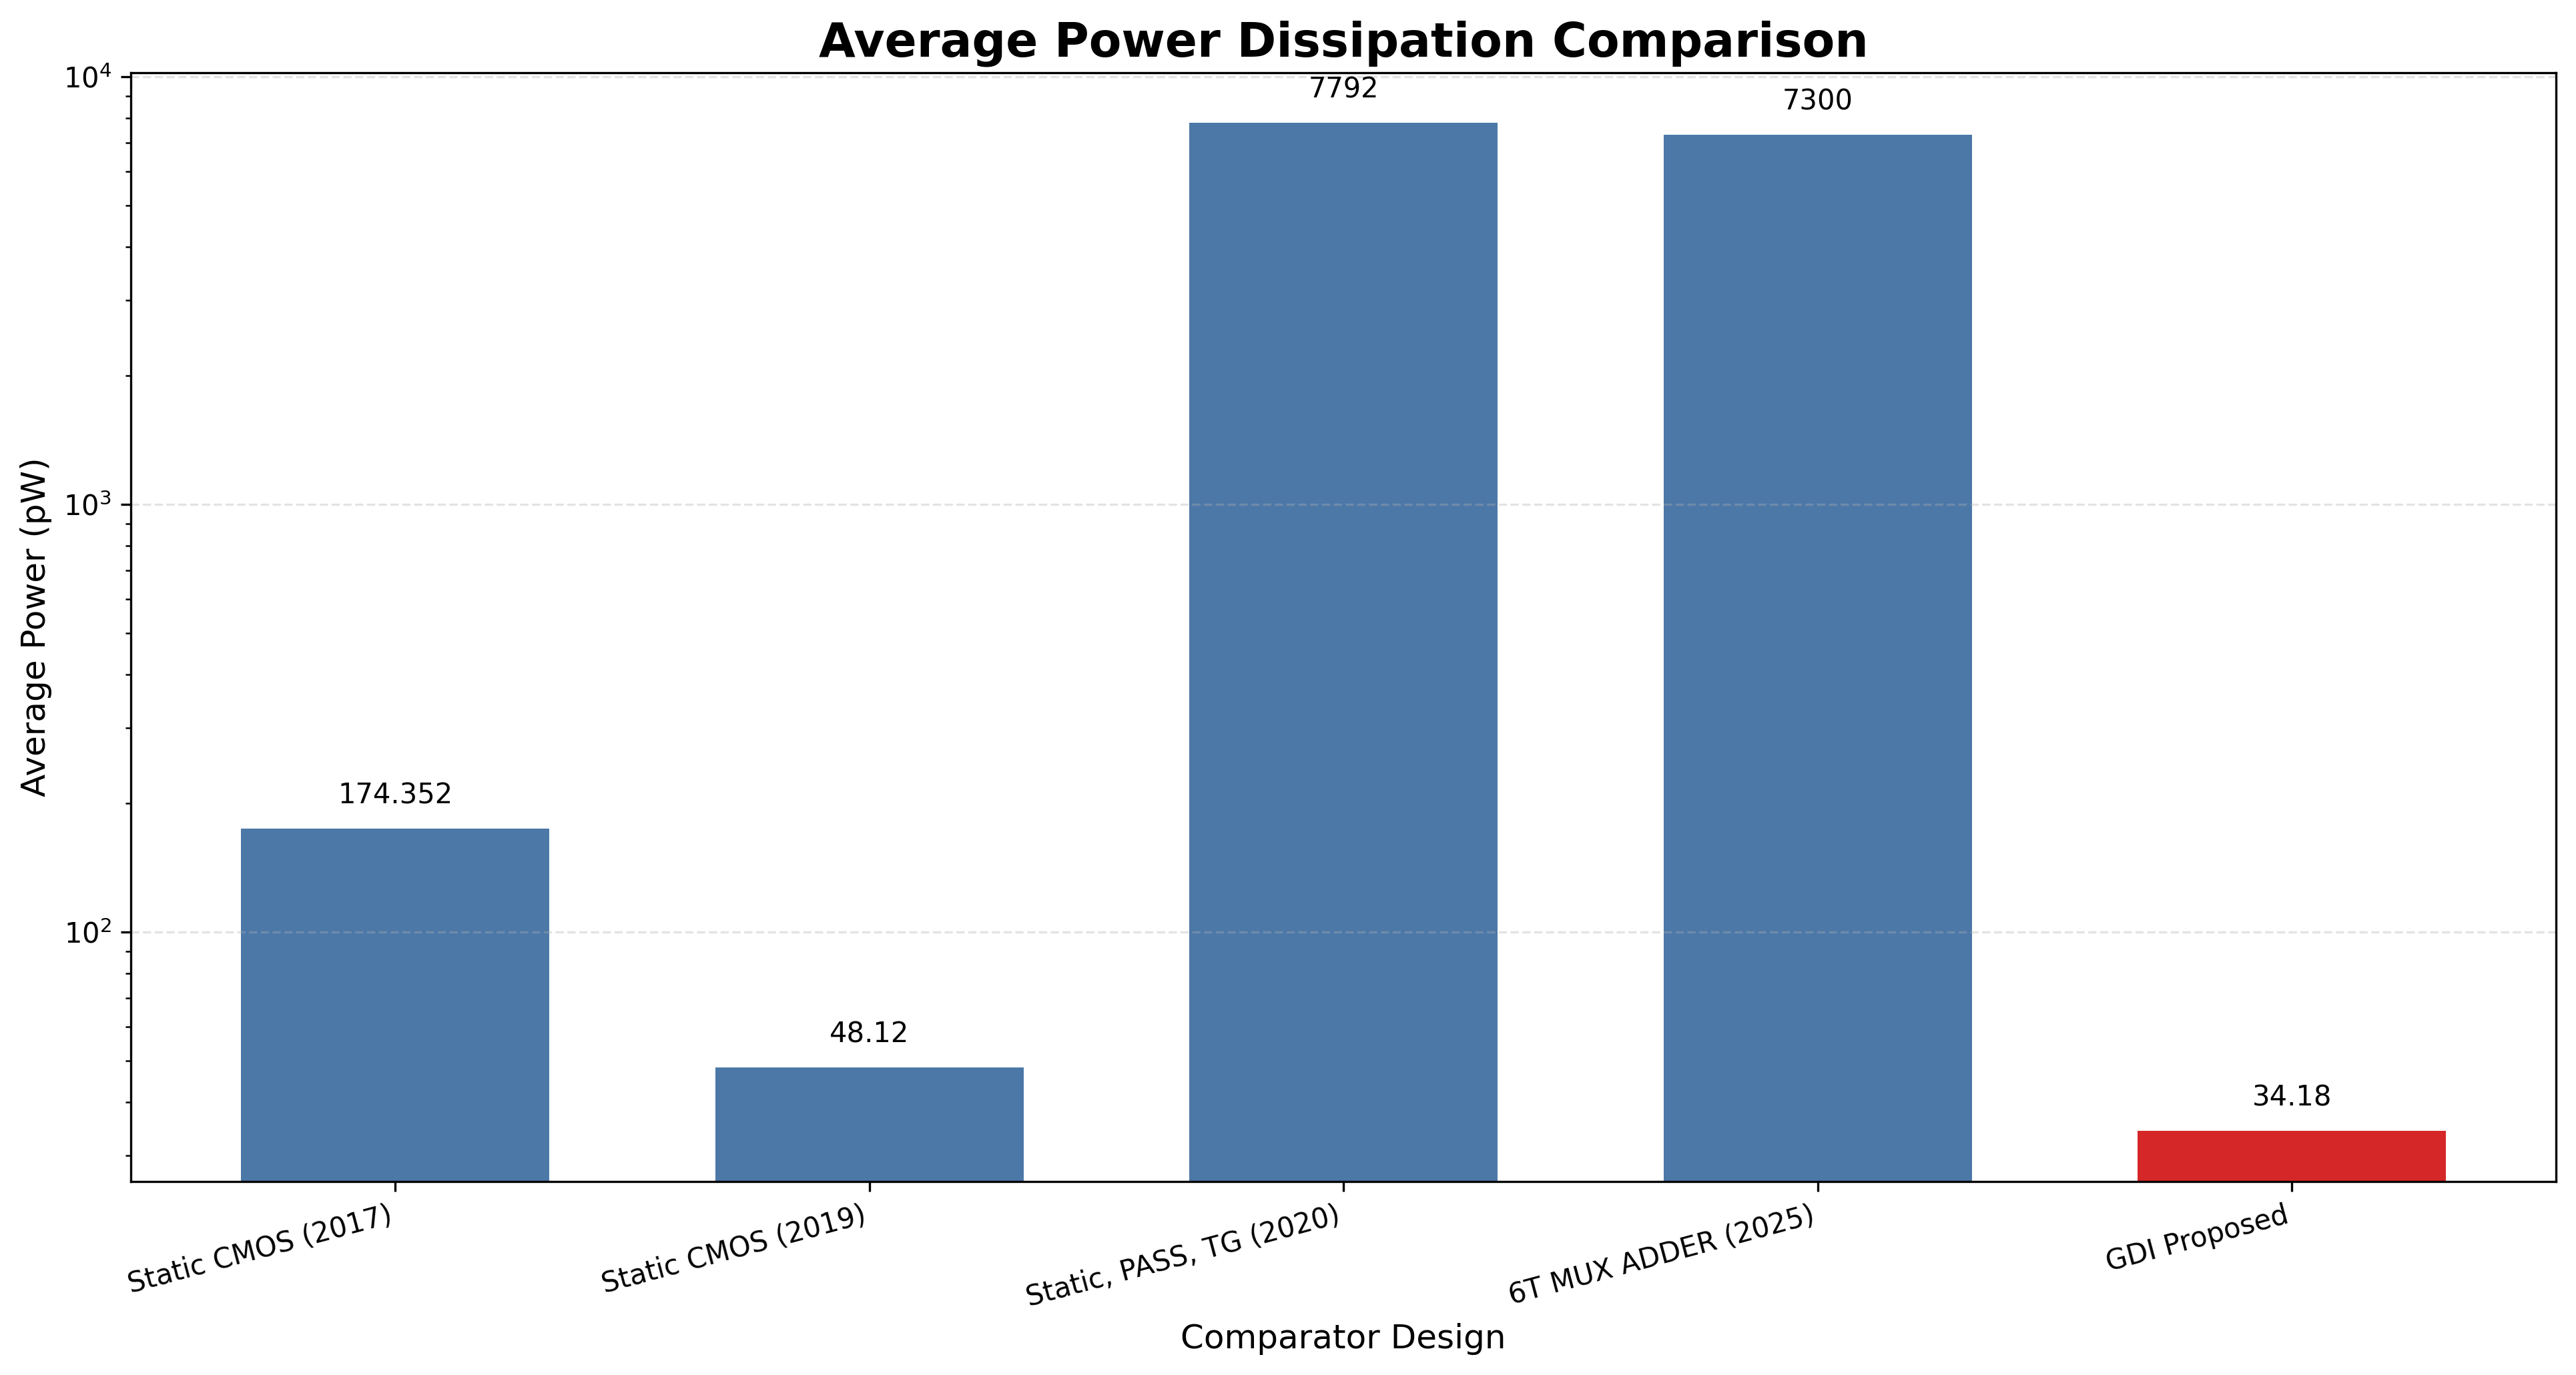
\includegraphics[width=\textwidth]{Paper_03_Average_Power_Bar_Chart.png}\\[0.1cm]
        \tiny Drastic reduction in parasitic capacitance.
      \end{block}
    \end{column}
    \begin{column}{0.32\textwidth}
      \begin{block}{Power-Delay Product}
        \centering
        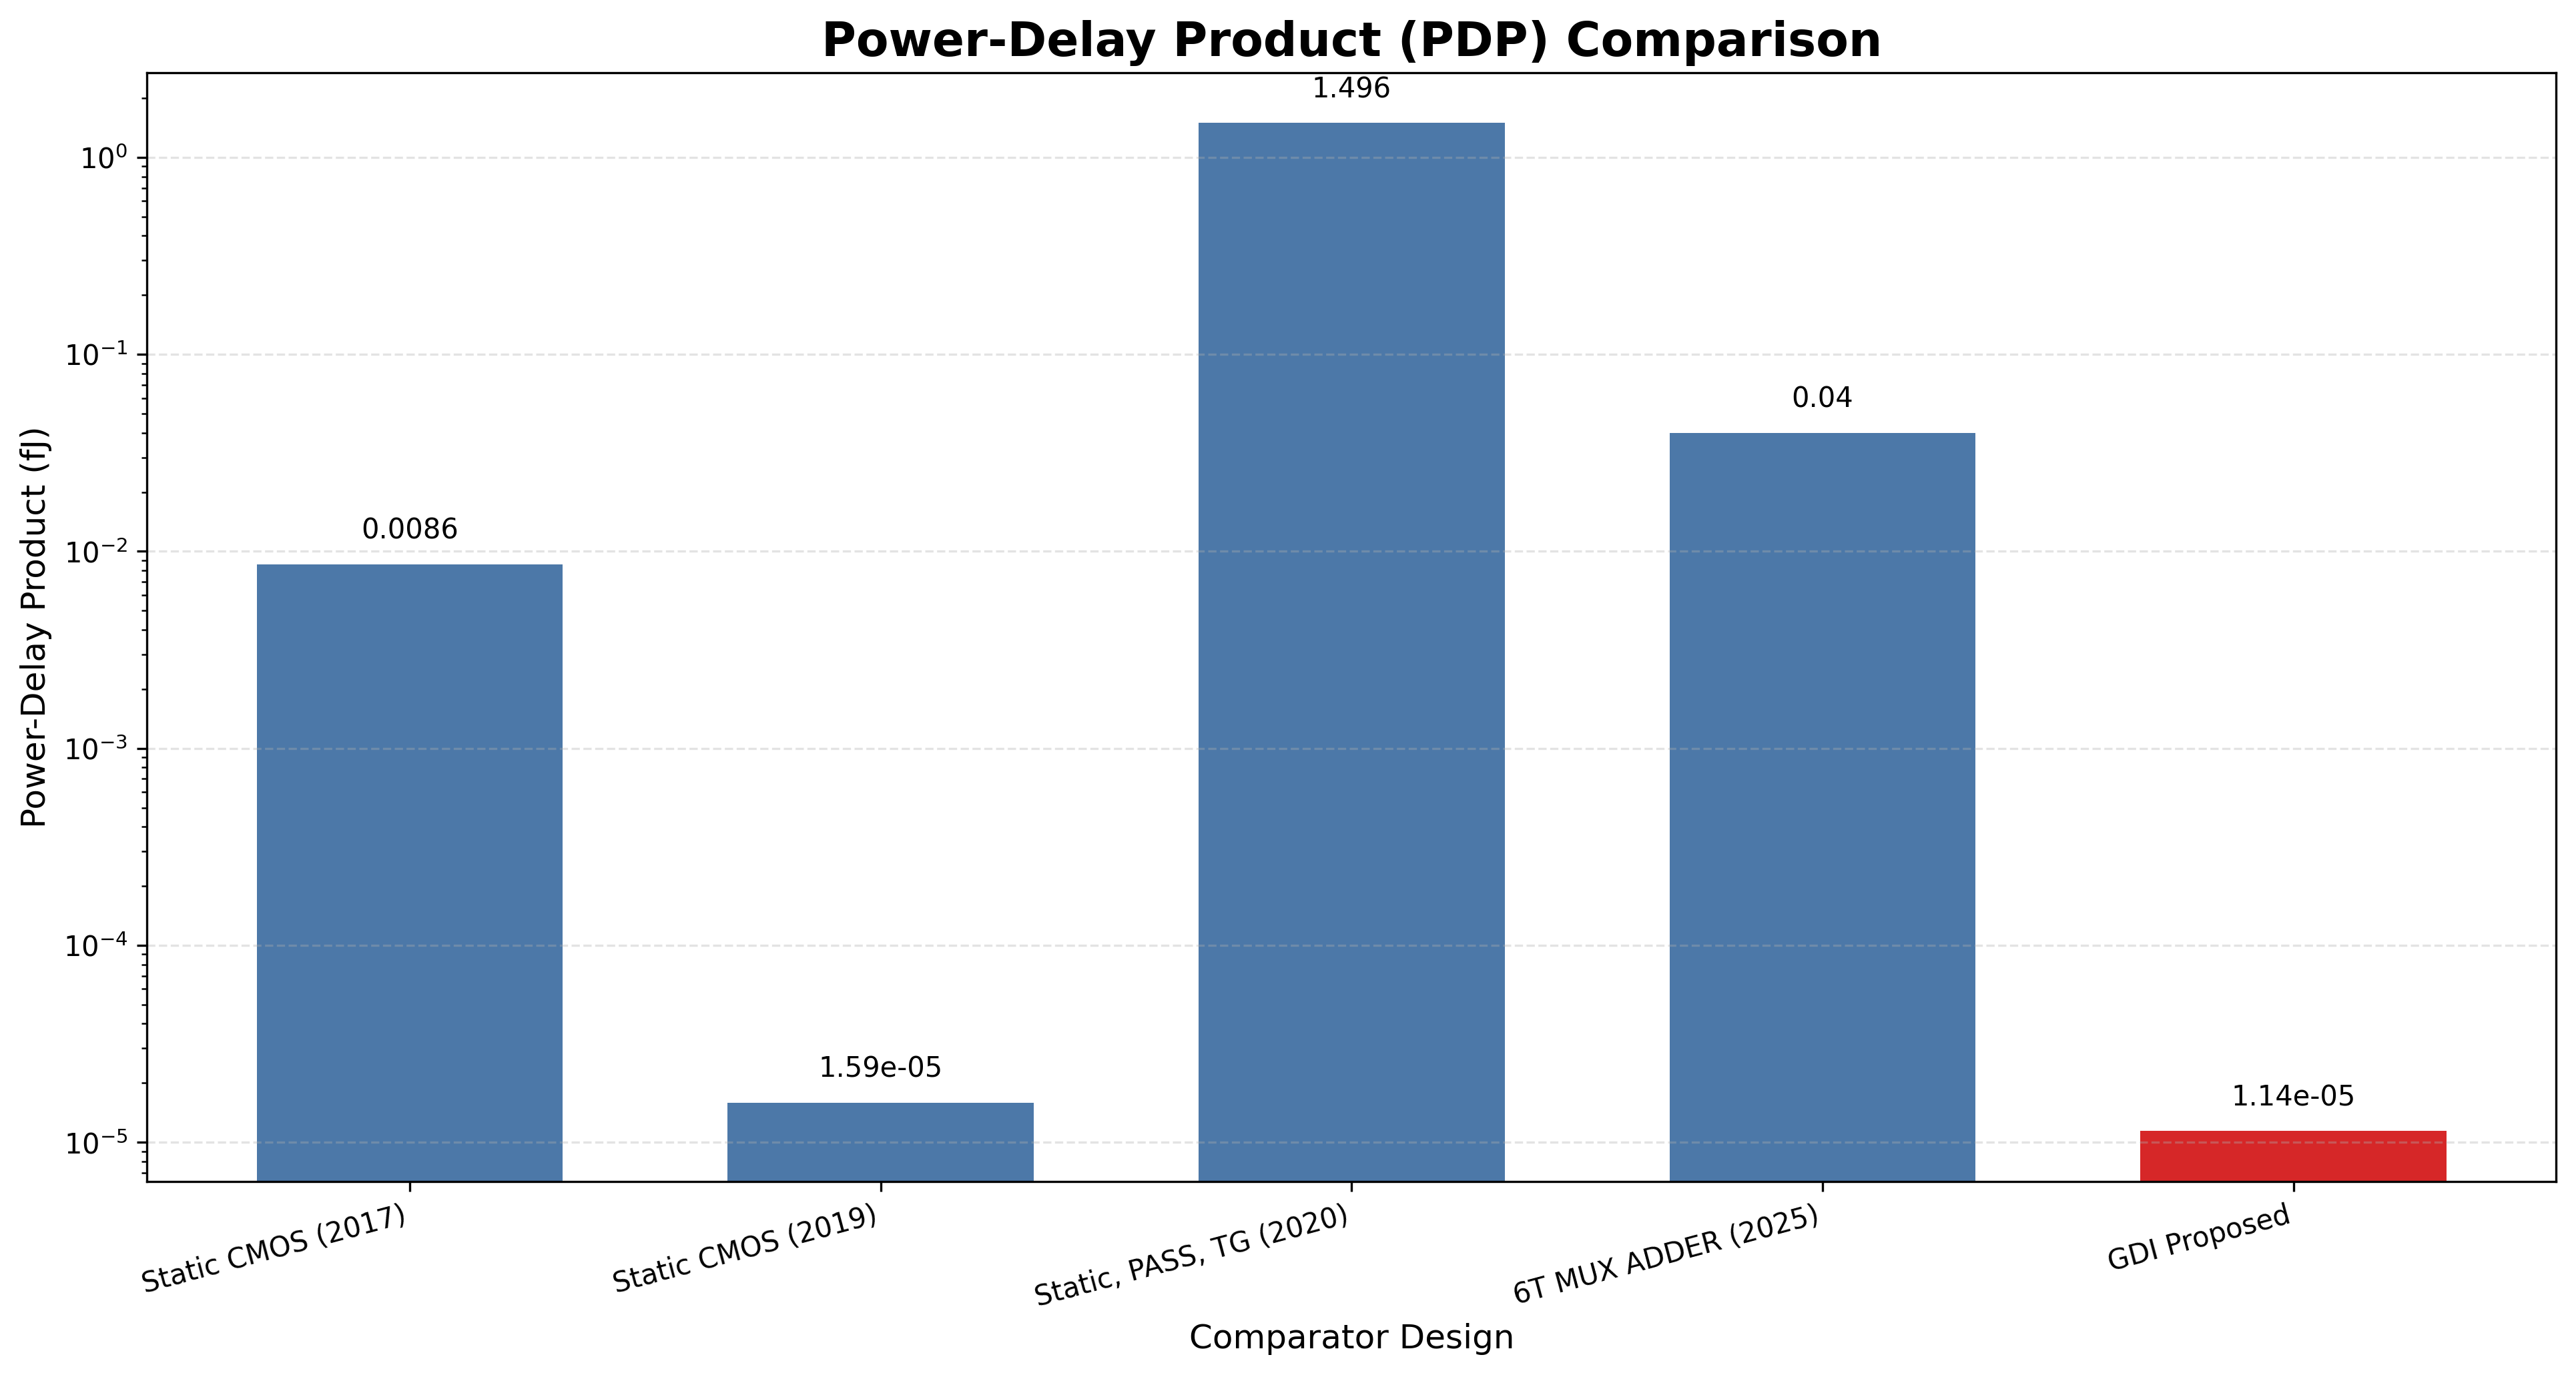
\includegraphics[width=\textwidth]{Paper_04_PDP_Bar_Chart.png}\\[0.1cm]
        \tiny Exceptional overall energy efficiency.
      \end{block}
    \end{column}
  \end{columns}
\end{frame}

% ============================================================================
\section{6. Conclusion \& Future Scope}
% ============================================================================

\begin{frame}{6. Conclusion \& Key Contributions}
  \begin{block}{Summary of Achievements}
    \begin{itemize}
      \item Designed and verified an ultra-low-power \textbf{10-Transistor 1-Bit Magnitude Comparator} using the GDI technique.
      \item Demonstrated superior scalability across \textbf{180nm, 90nm, and 45nm PTM nodes}.
      \item Achieved state-of-the-art performance with \textbf{$2.15\,\mu\text{W}$ power} and \textbf{$18.4\text{ ps}$ delay} at 45nm.
      \item Successfully solved transistor overhead without sacrificing output magnitude functionality.
    \end{itemize}
  \end{block}
  \pause
  \begin{block}{Future Scope \& Application Expansion}
    \begin{itemize}
      \item Scaling the 1-bit GDI comparator cell into \textbf{4-bit, 8-bit, and 32-bit high-speed ALU architectures}.
      \item Implementation with threshold-voltage swing restoration buffer stages for deep multi-bit cascading.
      \item Layout fabrication and Monte-Carlo corner analysis for PVT (Process, Voltage, Temperature) variations.
    \end{itemize}
  \end{block}
\end{frame}

\begin{frame}[plain]
  \centering
  \vfill
  {\Huge \textbf{\color{iiucblack} Thank You!}}\\[0.5cm]
  {\Large Questions \& Answers}\\[1cm]
  \begin{block}{\centering Contact Information}
    \centering
    \textbf{Shahrear Hossain} -- ID: ET223104\\
    Department of Electrical and Electronic Engineering\\
    International Islamic University Chittagong (IIUC)\\
    \small Email: shahrear@iiuc.ac.bd
  \end{block}
  \vfill
\end{frame}

\end{document}
